%%%%%%%%%%%%%%%%%%%%%%%%%%%%%%%%%%%%%%%%%
% Stylish Article
% LaTeX Template
% Version 2.1 (1/10/15)
%
% This template has been downloaded from:
% http://www.LaTeXTemplates.com
%
% Original author:
% Mathias Legrand (legrand.mathias@gmail.com) 
% With extensive modifications by:
% Vel (vel@latextemplates.com)
%
% License:
% CC BY-NC-SA 3.0 (http://creativecommons.org/licenses/by-nc-sa/3.0/)
%1
%%%%%%%%%%%%%%%%%%%%%%%%%%%%%%%%%%%%%%%%%

%--------------------------------------------------------------# Path to your oh-my-zsh installation.--------------------------
%	PACKAGES AND OTHER DOCUMENT CONFIGURATIONS
%----------------------------------------------------------------------------------------

\documentclass[fleqn,10pt]{SelfArx} % Document font size and equations flushed left

\usepackage[english]{babel} % Specify a different language here - english by default

\usepackage{marvosym, epigraph, subfig}

\usepackage[sortcites=false,style=authoryear-comp,bibencoding=utf8, natbib=true, firstinits=true, maxcitenames=2, maxbibnames = 99, uniquename=false, backend=bibtex, useprefix=true, backref=false,doi=false,isbn=false,url=false,dashed=true]{biblatex}
\setlength\bibhang{20pt}
\bibliography{ThomasReferenties.bib}
\AtEveryBibitem{%
	\clearfield{day}%
	\clearfield{month}%
	\clearfield{endday}%
	\clearfield{endmonth}%
}

%----------------------------------------------------------------------------------------
%	COLUMNS
%----------------------------------------------------------------------------------------

\setlength{\columnsep}{0.55cm} % Distance between the two columns of text
\setlength{\fboxrule}{0.75pt} % Width of the border around the abstract

%----------------------------------------------------------------------------------------
%	COLORS
%----------------------------------------------------------------------------------------

\definecolor{color1}{RGB}{0,0,90} % Color of the article title and sections
\definecolor{color2}{RGB}{0,20,20} % Color of the boxes behind the abstract and headings

%----------------------------------------------------------------------------------------
%	HYPERLINKS
%----------------------------------------------------------------------------------------

\usepackage{hyperref} % Required for hyperlinks
\hypersetup{hidelinks,colorlinks,breaklinks=true,urlcolor=color2,citecolor=color1,linkcolor=color1,bookmarksopen=false,pdftitle={What drives which region?},pdfauthor={Thomas de Graaff}}

%----------------------------------------------------------------------------------------
%	ARTICLE INFORMATION
%----------------------------------------------------------------------------------------

\JournalInfo{Research agenda, 2017--2021} % Journal information 
\Archive{Position paper} % Additional notes (e.g. copyright, DOI, review/research article)

\PaperTitle{Do regional economists answer the right questions?}
\SubPaperTitle{On the discrepancy between the questions regional economists solve and the questions policy makers actually ask}

\Authors{Thomas de Graaff\textsuperscript{1}*} % Authors
\affiliation{\textsuperscript{1}\textit{Department of Spatial Economics, Vrije Universiteit Amsterdam, Amsterdam, The Netherlands}} % Author affiliation
\affiliation{*\textbf{Corresponding author}: \Letter{} t.de.graaff@vu.n; \Mundus{} \href{thomasdegraaff.nl}{thomasdegraaff.nl}} % Corresponding author

\Keywords{Regional science --- spatial heterogeneity --- conditional robustness --- predicting --- data science}
\newcommand{\keywordname}{Keywords} 

%%----------------------------------------------------------------------------------------
%%	ABSTRACT
%%----------------------------------------------------------------------------------------

\Abstract{In this position paper I argue two things: namely, (\textit{i}) regional (or spatial) economists do not always answer the type of questions policy makers are concerned about, and consequently (\textit{ii}) they are very restrictive in the tool set they apply. First, policy makers---whether national, regional or local---are oftentimes concerned about holistic approaches and future predictions. Exemplary questions are ``What works best for my country/region/city'' and ``If we change this what will happen to the country/region/city as a whole?''. Regional economists---actually, most economists---usually isolate phenomena in order to, at best, explain the impact of a single determinant. Indeed, most regional economists feel very uncomfortable when asked to predict or give the best set of determinants for a certain phenomenon. This has its consequences for the tool set the regional economists applies. Usually a parametric regression type of framework is applied isolating the determinant under consideration and controlling as much as possible for observables and unobservables, ideally in a pseudo-experimental framework. A direct consequence of this approach is that emphasis is very much on explaining the impact of a determinant and not on predicting phenomena. For many applications that is definitely the right approach. However, as this paper ultimately argues, it is very much as well a selective approach that does not do well to deliver on some of the questions policy makers ask regional economists.}

%----------------------------------------------------------------------------------------

\begin{document}

\flushbottom % Makes all text pages the same height
\maketitle % Print the title and abstract box
\tableofcontents % Print the contents section
\thispagestyle{empty} % Removes page numbering from the first page

%----------------------------------------------------------------------------------------

\section*{Introduction: two different cultures} % The \section*{} command stops section numbering

\addcontentsline{toc}{section}{Introduction: two different cultures}

\epigraph{The sexiest job in the next 10 years will be statisticians.}{Hal Varian, 2009}

The above quote from Hal Varian is in one aspect wrong; nowadays, we do not call
them statisticians but data scientists instead. Nevertheless, in the last two
decades companies such as Google, Ebay, Whatsapp, Facebook, Booking.com and
Airbnb, have not only witnessed enormous growth but to a large extent also changed the socio-economic landscape. Indeed, with the increasing abundance of (spatial) data and computer capacity, the ability to gather, process, and visualize data has become highly important and therefore highly in demand as well. And all the models and tools these data scientists within these companies use are very much \textit{data driven} with often remarkable results. 

In his controversial and path-breaking article, \citet{breiman2001statistical}
presented two different cultures in statistical science. One governed by
a (probability) theory-driven modeling approach and one governed by a more (algorithmic) data-driven approach. These two cultures carry over to the econometric and ultimately the
empirical regional economics domain\footnote{I use a wide definition for the regional economics
 domain, which consists of most aspects of regional science in general but for
 which the theoretical approach is always from an economic perspective. Topics
 such as, e.g, interregional migration, trade, transport flows and commuting on
 the one side and regional performance, clustering, population growth and
 specialisation on the other side fall all under this, admittedly, rather wide umbrella.} as well, where---commonly for all social
science---the theory driven approach still very much dominates the landscape of the realm of regional economics of today. 

\begin{figure*}[h!]\centering 
	\subfloat[Modeling approach\label{modelapproach}]{%
		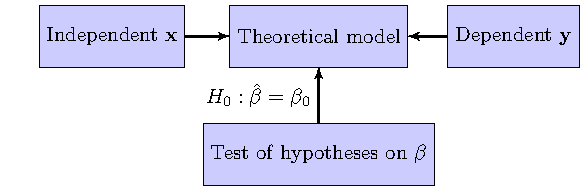
\includegraphics[width=0.49\textwidth]{./figures/modelapproach}
	}
	\hfill
	\subfloat[Data approach\label{dataapproach}]{%
		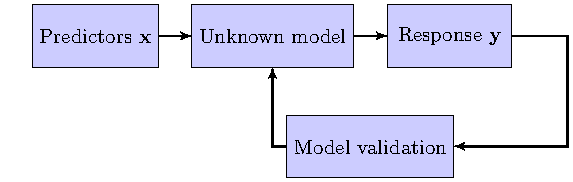
\includegraphics[width=0.49\textwidth]{./figures/dataapproach}
	}
0	
	\caption{Two cultures of statistical/econometric modeling \citep[inspired by][]{breiman2001statistical}}
	\label{fig:twocultures}
\end{figure*}

Figure \ref{fig:twocultures} is an adaptation from the one displayed in \citet{breiman2001statistical} and describes the processes governing these two cultures. Figure (\ref{modelapproach}) is what I refer to as the modeling approach, where a statistical model is postulated and is central to this culture. This is the classical approach\footnote{Sometimes as well referred to as the frequentists' approach. However, this typically concerns the debate between classical statistics and Bayesian statistics, where the two approaches I refer to are more concerned with wider frameworks, of which the Bayesian approach is just one of the elements.} where statistical probability theory meets the empiricism of Karl Popper. Usually the model assumed is stated as a linear model and in its most simple form can be denoted as:
\begin{equation}
	\mathbf{y} = \mathbf{x}\beta + \epsilon, 
\end{equation}
where in (regional) economics language, $\mathbf{x}$ is referred to as the
independent variable, $\mathbf{y}$ as the dependent variable and $\epsilon$ as a
residual term. In this setup, using the data at hand, one typically constructs a
statistical test to which extent the estimated coefficient (denoted with
$\hat{\beta}$) deviates from a hypothesized value of the coefficient (denoted
with $\beta_0$)---typically the hypothesis $H_0: \hat{\beta} = 0$ is used with
as alternative hypothesis that $H_1: \hat{\beta} \neq 0$. However, that is
always within the context of the \textit{postulated} model. So, when the
null-hypothesis is rejected, it not necessarily means that the true $\beta$ is
unequal to zero, it might also be caused by errors in measuring $\bf{x}$ or even using the wrong \textit{model}!\footnote{One of the assumptions for regression techniques such as the one used here is actually no misspecification of the model, but---apart from some possible tests on the functional form \textit{within} a specific regression form---usually little attention is give on the validity of the model used. More importantly, within this framework the model itself is usually not tested \textit{a posteriori}.}

Therefore it is striking that in economics in general, and in regional economics
in specific, most of the tools employed are very much \textit{theory or model driven} instead of data driven. My (conservative) estimate would be that 90\% of all empirical work in regional economics revolves around postulating a (linear) model and testing whether (a) key determinant(s) are significantly different from a hypothesized value---usually zero.\footnote{In a seminal contribution, \cite{breiman2001statistical} states that deep into the 90s 98\% of the statisticians actually employed the theory driven paradigm and only 2\% a data driven paradigm. With the advent of the availability of internet connectivity, large (online) data sources, and faster computers the statistical realm changed dramatically. However, this has not permeated yet in the social sciences.} That is, \textit{within} the context of the model assumed.

At best, this approach can be seen in a causal inference framework. If a
determinant (such as a policy in the context of economics) $x$ changes, does it
cause then a change in the output $y$ (most economists typically use some welfare measure).\footnote{Most of this research actually intends to mimic a \textit{difference-in-difference} approach and gained enormous momentum with the textbook of \citet{angrist2008mostly}.} This approach thus provides a rigid and useful approach to regional policy evaluation. If we implement policy $x$, does welfare measure $y$ then improve? 

However, policy makers oftentimes have different questions for which they need
solutions. Usually, they revolve around questions starting with \textit{``What
  determines performance measure $A$?''} or, more generally, \textit{``What
  works for my region?''}. These types of questions require a different approach
than the previous one. Namely, the former type requires an approach focused on \textbf{explaining} while the latter type requires an approach focused on \textbf{predicting}.

The remaining part of this position paper is structured as follows. The next
section deals with the historical background both from an applied statistical
and econometric point of view and from a regional science point of view. Section
\ref{practices} deals with current practices and describes the `traditional'
inference based approach as well as some data-driven approaches that have been
used in the recent past (though by far not as often as the traditional methods).
Section \ref{agenda} sets out both a research and an education agenda as it
addresses how to bridge the gap between the daily practices of regional
economists and the demands of local policy makers. The final section shortly
summarizes the main points raised in this position paper.  

%------------------------------------------------

\section{The road to current day's practice in regional economics\label{Background}}

Why do we do it as we do it?

%------------------------------------------------

\section{Regional economists turning the blind eye\label{practices}}

\subsection{The blind eye in research}

Regions are conceptually different than cities, as they contain urban, suburban and rural areas simultaneously. Whilst smaller regions can still be seen as the total influence radius of metropolitan areas---such as measured by the concept of local labor markets and the NUTS-2 regions in Europe---, larger regions can typically contain a multiple of cities in combinations with their various hinterlands --such as the Dutch Randstad, the Belgian Flemish Diamond, and the German Ruhr areas. 

In recent years, the urban economics literature witnessed large growth; not only noticed by a wider acceptance in mainstream economics, but as well by larger scientific rigor and increased robustness of empirical findings. Remarkably, the empirical regional economics (or regional science in general for that matter) literature lagged behind, although many concepts and challenges in both disciplines are conceptually similar and are derived from similar theoretical backgrounds. 

Similar to urban economics, there is not yet a clear (consensus in) understanding in which policy instruments are actually (cost-)effective in promoting regional growth. 

To do so, I first review the previous literature in section \ref{Background}. This section focuses mainly on regional economics as it has a larger emphasis on \textit{causal} effects. To a lesser extent we deal with the (economic geography) literature. Based on this literature review Section \ref{gaps} deals with the research gaps that can be identified.


\begin{itemize}
	\item housing \& population; 
	\item amenities;
	\item connectivity \& accessibility
	\item networks;
	\item social \& humn capital
\end{itemize}

\subsection{The blind eye in education}

%------------------------------------------------

\section{Incorporating the data science culture\label{agenda}}

What do we need?

\subsection{For research}

\subsubsection{Regional heterogeneity}

\citep{Thissen2016, Graaff2012, DeGraaff2012}

\subsubsection{Conditional robustness}

In regional science in general and in regional economics in specific, remarkably little attention has been given to reproducibility and robustness of results \citep[with some exceptions as, amongst some others, by][]{Rey:2014cl,arribas2015woow, Arribas2016}.

\subsubsection{Regional sorting models}

As in \citet{Bayer2004, Bayer2007a} and recently by \citet{Wang2016} and \citet{Bernasco2016}.

\subsection{For education}

\section{From here to eternity}

%----------------------------------------------------------------------------------------
%	REFERENCE LIST
%----------------------------------------------------------------------------------------

\addcontentsline{toc}{section}{References} % Adds this section to the table of contents
\printbibliography

%----------------------------------------------------------------------------------------

\end{document}